La Organización Europea para la Investigación Nuclearo \CERN (\textbf{C}onseil \textbf{E}uropéen pour la \textbf{R}echerche \textbf{N}ucléaire) es una organización de investigación europea que opera el laboratorio de física de partículas más grande del mundo, está situado en Suiza cerca a la frontera con Francia, entre la comuna de Saint-Genis-Pouilly y la comuna de Meyrin. La función principal del \CERN ~ es proporcionar los aceleradores de partículas y otra infraestructura necesaria para la investigación de física de alta energía; como resultado, se han construido numerosos experimentos en el \CERN ~ a través de colaboraciones internacionales. El sitio principal de Meyrin alberga una gran instalación informática, que se utiliza principalmente para almacenar y analizar datos de experimentos, así como para simular eventos. Los investigadores necesitan acceso remoto a estas instalaciones, por lo que el laboratorio ha sido históricamente un importante centro de red de área amplia. En la Fig. \ref{cern} se muestra un diagrama de las instalaciones y los proyectos en los que está dividido. 

El \CERN ~ es fundamentalmente un conjunto interconectado de aceleradores de partículas cuyo primer elemento, el Sincro-Ciclotrón de protones o \textbf{SC} (\textbf{S}ynchro-\textbf{C}yclotron) se empiezó a construir a mediados de 1955, sustituido por el Gran Coalisión de Hadrones  o \LHC (\textbf{L}arge \textbf{H}adron \textbf{C}ollider) puesto en funcionamiento el 2008. En la actualidad, gran parte de la actividad experimental que se realiza en el \CERN ~ está concentrada en la construcción de los experimentos para el \LHC:
\begin{itemize_f}
\item \textbf{ATLAS} (\textbf{A T}oroidal \textbf{L}HC \textbf{A}pparatu\textbf{S}) : Investiga una amplia gama de física, desde la búsqueda del bosón de Higgs hasta dimensiones adicionales y partículas que podrían formar materia oscura. Aunque tiene los mismos objetivos científicos que el experimento \CMS, utiliza diferentes soluciones técnicas y un diseño de sistema magnético diferente. Página del proyecto : \href{https://atlas.cern}{https://\-atlas\-.\-cern}%\url{https://home.cern/science/experiments/atlas} %~~~~~~~~~~~~~~~~~~~~~~~~~~~~~~~~~

\item \CMS \href{https://en.wikipedia.org/wiki/Compact_Muon_Solenoid}{(\textbf{C}ompact \textbf{M}uon \textbf{S}olenoid) :} Tiene un amplio programa de física que va desde el estudio del Modelo estándar (incluido el bosón de Higgs) hasta la búsqueda de dimensiones y partículas adicionales que podrían formar materia oscura. Está construido alrededor de un gran imán de solenoide. Página del proyecto : \href{https://cms.cern/detector}{https://\-cms.\-cern/\-de\-tec\-tor}%\url{https://home.cern/science/experiments/cms} %~~~~~~~~~~~~~~~~~~~~~~~~~~~~~~~~~

\item \href{https://es.wikipedia.org/wiki/LHCb}{\textbf{LHCb} (\textbf{L}arge \textbf{H}adron \textbf{C}ollider \textbf{b}eauty) :} experimento especializado en física del \quark ~ b, algunos de cuyos objetivos son la medida de parámetros de violación de simetría \textbf{CP} en las desintegraciones de hadrones que contengan dicho \quark ~ o la medida de precisión de las fracciones de desintegración (``branching ratios'') de algunos procesos extremadamente infrecuentes. Página del proyecto: \href{http://lhcb-public.web.cern.ch/lhcb-public}{http://lhcb-\-public.\-web.\-cern.\-ch/\-lhcb-\-public}

\item \href{https://en.wikipedia.org/wiki/ALICE_experiment}{\textbf{ALICE} (\textbf{A L}arge \textbf{I}on \textbf{C}ollider \textbf{E}xperiment) :} es un detector de iones pesados, estudiar la física de la materia que interactúa fuertemente a densidades de energía extremas, donde se forma una fase de la materia llamada plasma quark-gluón. Página del proyecto: \href{http://aliceinfo.cern.ch/Public/Welcome.html}{http://aliceinfo\-.cern\-.ch/\-Public/\-Welcome\-.html}

%\item[-] \href{https://en.wikipedia.org/wiki/Proton_Synchrotron}{\textbf{PS} (\textbf{P}roton \textbf{S}ynchrotron) :} es un componente clave en el complejo acelerador del \CERN, donde generalmente acelera los protones suministrados por el Proton Synchrotron Booster o los iones pesados del Anillo de iones de baja energía (LEIR). En el curso de su historia, ha hecho malabarismos con muchos tipos diferentes de partículas, alimentándolas directamente a experimentos o aceleradores más potentes.

%\item[-] SPS
\end{itemize_f}

\begin{figure}[h!]
\centering
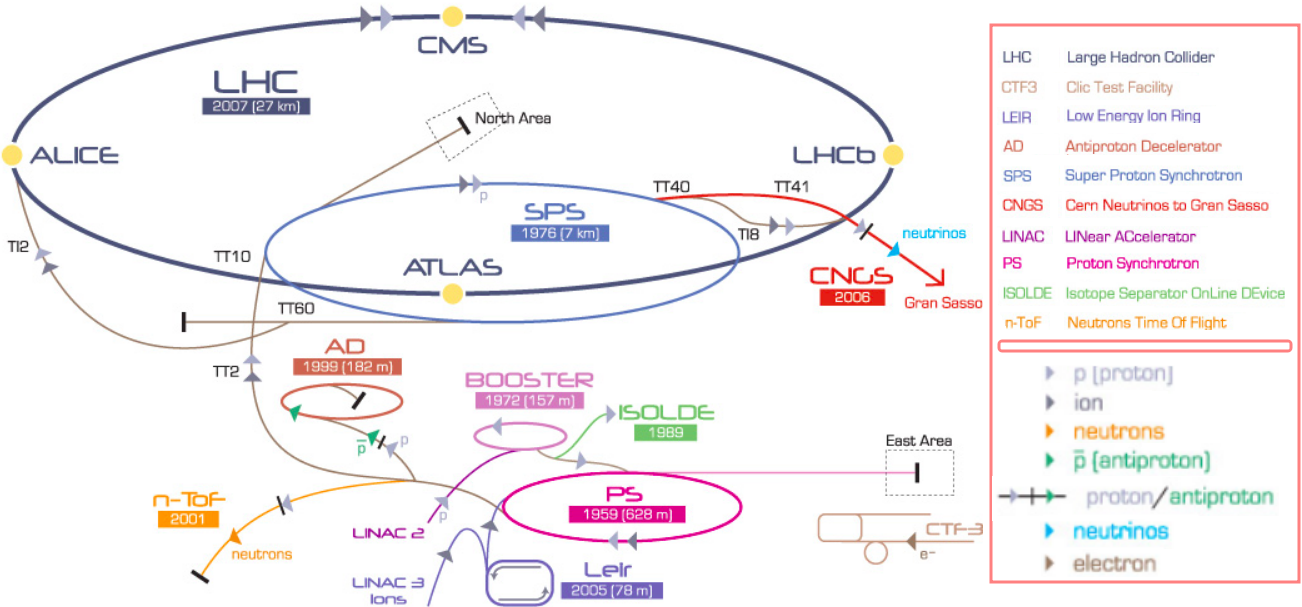
\includegraphics[width=.9\textwidth]{Analisis_y_Resultados/imagenes/cern.png}
\caption[Diagrama de los experimentos que componen el centro de investigación del \CERN.]{Diagrama de los experimentos que componen el centro de investigación del \CERN.\footnotemark}
    \label{cern}
\end{figure}
\footnotetext{Página de origen: \href{https://theconversation.com/goodbye-for-a-while-to-the-large-hadron-collider-12238}{https://\-the\-con\-ver\-sa\-tion.\-com/\-goodbye-\-for-\-a-\-while-\-to-\-the-\-large-\-hadron-\-collider-\-12238}}

Uno de los experimentos considerado por sus resultados de los mas importantes es el \CMS, el cual es uno de los detectores multi-usos del \CERN ~ como se puedo constatar anteriormente, dicho detector tiene la capacidad de cubrir un amplio rango de procesos físicos, siendo este junto con el experimento \textbf{ATLAS} los que reportaron la observación de la partícula de Higgs en el 2012. El mismo es uno de los recursos principales para las investigaciones relacionadas con la exploración de la materia oscura.

El experimento \LHC ~está continuamente en proceso de actualización con el objetivo de proporcionar mediciones más precisas de nuevas partículas y permitiendo observar raros procesos teorizados y de esta intentar aumentar  nuestros conocimientos de la materia oscura. Esto se debe a que el número de eventos de un dado proceso producidos en un colisionador está dado por:
\begin{equation}
N = L \sigma
\end{equation}
donde $\sigma$ es la sección eficaz del proceso físico y $L$ es la luminosidad integrada del acelerador.

La luminosidad instantánea es uno de los parámetros más importantes para caracterizar el funcio­namiento del acelerador, definida como el número de partículas (protones o iones pesados en el caso del \LHC) por unidad de tiempo y unidad de área, y puede calcularse mediante la relación:
\begin{equation}
\mathcal{L} = f_\mathbf{rev} n_b \dfrac{\mathbf{N}_1 \mathbf{N}_2}{\mathbf{A}}
\end{equation}
donde $f_\mathbf{rev}$ es la frecuencia de revolución, $n_b$ es el número de bunches (paquetes de protones) por haz, $\mathbf{N}_i$ es el número de partículas en cada bunch y $\mathbf{A}$ es la sección efectiva del haz, que puede expresarse en término de los parámetros del acelerador como:
\begin{equation}
A = \dfrac{4 \pi \epsilon_n \beta^*}{\gamma \mathbf{F}}
\end{equation}
donde $\epsilon_n$ es la emitancia transversal normalizada (la dispersión transversal media de las partículas del haz en el espacio de coordenadas e impulsos), $\beta^*$ es la función de amplitud en el punto de interacción, relacionada al poder de focalización de los cuadrupolos), $\gamma$ es el factor relativista de Lorentz y $\mathbf{F}$ es un factor de reducción geométrico, debido al ángulo de cruce de los haces en el punto de interacción.


\subsection{Actualizando LHC}
El programa de línea de base del \LHC~ tenía el objetivo de producir los primeros resultados en la carrera 2010-2012 con el objetivo de una \href{https://es.wikipedia.org/wiki/Luminosidad}{luminosidad integrada} de al menos $1~fb^{-1} = 40~m^2$ para fines de 2011 y gracias a un rendimiento mejor de lo previsto se obtuvo más de $25~fb^{-1}$ en colisión de $pp$ a finales de 2012, más allá de cualquier expectativa. Después se alcanzó la energía de $13-14 ~ \textbf{TeV}$ de centro de masa de energía en 2015.

Después de 2019, la ganancia estadística al ejecutar el acelerador sin un aumento considerable de luminosidad más allá de su valor de diseño fue más de la prevista. El tiempo de ejecución necesario para reducir a la mitad el error estadístico en las mediciones. Por lo tanto, para mantener el progreso científico y explorar su capacidad total, el \LHC ~ necesitará un aumento decisivo de su luminosidad. Por eso, cuando el Consejo del \CERN ~ adoptó la Estrategia Europea para la Física de Partículas en Bruselas el 30 de mayo de 2013, se acordó que su primera prioridad sería:

\begin{minipage}{0.9\linewidth}
\vspace{5pt}%margen superior de minipage
{\small }
\textit{``La máxima prioridad de Europa debería ser la explotación de todo el potencial del \LHC, incluido el actualización de alta luminosidad de la máquina y los detectores con el fin de recopilar diez veces más datos que en el diseño inicial, alrededor de 2030''}
\begin{flushright}
cita traducida de la referencia \cite{wells_upgraded_2015}
%(\citeauthor{Coulouris}, \citeyearNP{Coulouris}: 10)
\end{flushright}
\vspace{5pt}%margen inferior de la minipage
\end{minipage}

Además se reemplazarán los imanes triples internos (el responsable de exprimir el rayo en caso de colisión) y de todos los cambios de hardware necesarios para permitir una ambiciosa actualización de luminosidad. Con algunas de las modificaciones ya cumplidas en 2019 ($LS2$), esta nueva fase de la vida del \LHC ~ se ha denominado ``\LHC ~ de alta luminosidad'' (\textbf{HL-}\LHC) y tiene la aspiración de alcanzar el sorprendente umbral de $3000~fb^{-1}$ en 10-12 años, entregarando hasta la actualización aproximadamente $\backsim 300~fb^{-1}$ durante ese período (ver Fig. \ref{cms_actualiza}).


\begin{figure}[h!]
\centering
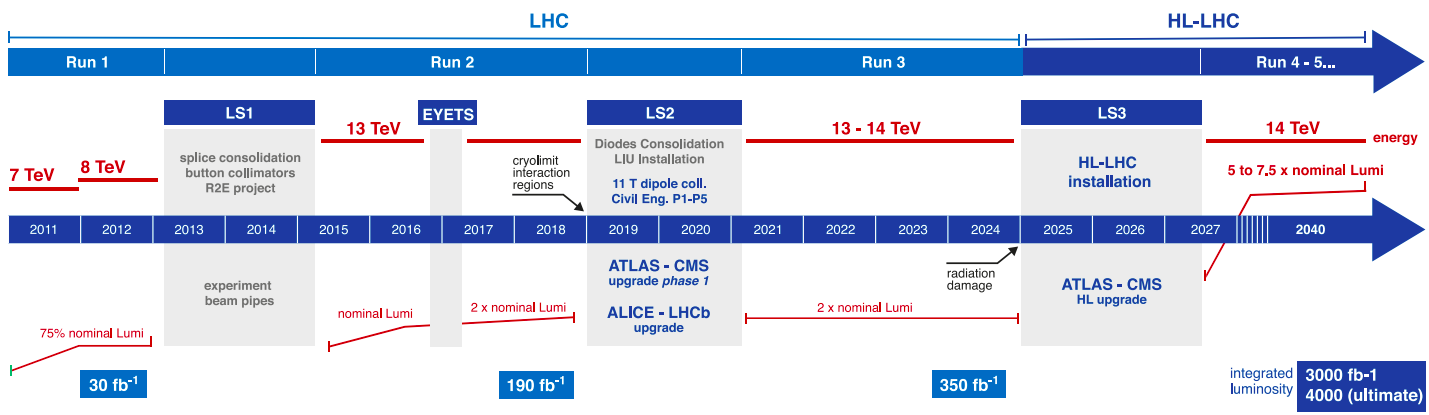
\includegraphics[width=1\textwidth]{Analisis_y_Resultados/imagenes/CMS_upgrade.png}
\caption[Plan de actualización del experimento \LHC.]{Plan de actualización del experimento \LHC.\footnotemark}
\label{cms_actualiza}
\end{figure}

\footnotetext{Página de origen: \href{https://hilumilhc.web.cern.ch/content/hl-lhc-project}{https://\-hilumilhc.\-web.\-cern.\-ch/\-content/\-hl-\-lhc-\-project}}

Con la actualización del \LHC ~se espera aumentar los conocimiento más allá del Modelo Estándar y su bosón de Higgs, siendo sus apuestas a la misteriosa materia oscura, con la teoría de la supersimetría. Pero para lograr actualizar una maquinaria tan compleja a tan gran escala se planifica una década en completarse. El proceso depende de una serie de tecnologías innovadoras que el proyecto \textbf{HL-}\LHC ~ está explorando. Esta extraordinaria empresa técnica dependerá de una combinación de imanes superconductores de vanguardia, cavidades de radiofrecuencia superconductoras compactas y ultraprecisas para la rotación del haz, así como enlaces superconductores de alta potencia de $100 ~m$ de largo con disipación de energía cero. Además, las altas luminosidades generarán nuevas demandas de vacío, criogenia y protección de la máquina, y requerirán nuevos conceptos para la colimación y el diagnóstico, modelado avanzado para el haz intenso y nuevos esquemas de cruce del haz para maximizar la salida física de las colisiones.




